%\chapterimage{Geometrijska.jpg} % Chapter heading image

\chapter{Interferenca}
\label{chap:Interferenca}
Spoznali bomo, da sta uklon in interferenca tesno povezana in pravzaprav
manifestacija istega pojava -- seštevanja  valovanj v 
skupno optično polje. V poglavju o uklonu so nas zanimali predvsem uklonski 
vzorci, v poglavju o interferenci pa se bomo osredotočili na interferometrijo 
in pojave na tankih plasteh.

\section{Interferenca in interferometrija}
O interferenci govorimo, kadar je na danem mestu v 
prostoru jakost električnega polja sestavljena iz 
več valovanj. Seštevanje 
dveh ali več valovanj ponekod vodi
do ojačevanja svetlobe (konstruktivna interferenca), 
drugod pa do oslabitev (destruktivna interferenca). 
Vzorci izmenjujočih se ojačitev in oslabitev sestavljajo
značilno interferenčno sliko.

Elektromagnetna valovanja se na splošno razlikujejo 
v smeri širjenja, amplitudi, frekvenci, fazi ali polarizaciji. 
Spoznali bomo, da se interferenčna slika pojavi le pri valovanjih z enako
polarizacijo, konstantno (ali zelo počasi se spreminjajočo)
začetno fazo in enako (oziroma približno enako) frekvenco. 
Če se frekvenci valovanj ne ujemata, se svetlobno valovanje na 
danem mestu zelo hitro spreminja in slika, ki jo zaznamo, se izpovpreči.
Zahteva o konstantni fazi je povezana s koherenco valovanja, 
ki jo bomo podrobneje obravnavali v poglavju~\ref{chap:Koherenca}. 

Najpreprostejši interferenčni poskusi so taki, pri katerih vpadni snop svetlobe
razdelimo na več delov. To lahko naredimo z delitvijo po valovni fronti
ali z delitvijo po amplitudi. V obeh primerih so zahteve po isti frekvenci, 
polarizaciji in začetni fazi izpolnjene, seveda pa se valovanji razlikujeta 
v dodatnem faznem zamiku, ki ga pridobita po delitvi.
Dodatni fazni zamik in z njim povezana interferenčna slika 
sta močno odvisna od dolžine poti, ki jo prepotuje del prvotnega snopa 
vpadne svetlobe. Ker je valovna dolžina svetlobe zelo majhna, že majhne 
spremembe v dolžini poti oziroma zakasnitvi žarka povzročijo velike spremembe 
interferenčnega vzorca. 

Z opazovanjem interferenčnih vzorcev lahko zelo natančno določimo fazni zamik med
dvema deloma valovanja in s tem pridobimo podatke o valovanju samem, o snovi, po 
kateri se širi valovanje, ali o oddaljenosti predmeta, od katerega se svetloba odbija. 
Zato interferometrijo, kot imenujemo metodo, ki temelji na opazovanju interference,
s pridom uporabljamo med drugim za izredno natačne meritve dolžine, 
oddaljenosti, lomnega količnika snovi oziroma njegovih sprememb ali odstopanj v frekvenci. 
Interferenčne meritve so ene najnatančnejših in so zato zelo uporabne na veliko področjih:
od prvotne opustitve obstanka etra prek izredno natačnih meritev gladkosti površine do
opazovanja gravitacijskih valov. 

V laboratorijih in industrijskih aplikacijah navadno za vir svetlobe uporabljamo laser, zato
je interferenčna slika sestavljena iz svetlih in temnih območij. V naravi interferenco
navadno opazujemo z belo dnevno svetlobo, kar da snovem, na primer plasti olja na vodi ali
milnemu mehurčku, značilno mavrično obarvanost.

\section{Interferenca dveh ravnih valov}
Zapišimo preprost primer interference dveh ravnih valov z enako frekvenco. Valovna
vektorja valovanj označimo s $\mathbf{k}_1$ in $\mathbf{k}_2$, fazi valovanj z 
$\delta_1$ in $\delta_2$ ter njuni realni amplitudi z $E_{10}$ in $E_{20}$. Ker imajo 
valovanja, ki interferirajo, isto polarizacijo,
za račun interference zadošča skalarna oblika električnega polja.
Valovanji potem zapišemo kot:
\beq
E_1 = E_{10} e^{i\mathbf{k}_1 \cdot \mathbf{r} - i \omega t + i \delta_1}
\qquad \mathrm{in} \qquad
E_2 = E_{20} e^{i\mathbf{k}_2 \cdot \mathbf{r} - i \omega t + i \delta_2}.
\label{eq:06_01}
\eeq
Celotno
električno polje je vsota obeh prispevkov:
\beq
E = E_1 + E_2 = E_{10} e^{i\phi_1 - i \omega t} + E_{20} e^{i\phi_2 - i \omega t},
\label{eq:06_02}
\eeq
pri čemer sta $\phi_{1,2} = \mathbf{k}_{1,2} \cdot \mathbf{r} + \delta_{1,2}$. 
Gostota svetlobnega toka $j$ je na splošno (enačba~\ref{eq:j}):
\beq
j = \frac{1}{2}\varepsilon \varepsilon_0 |E|^2c,
\label{eq:06_03}
\eeq
zato je celotna gostota svetlobnega toka enaka:
\beq
j \propto (E_1+E_2)(E_1^*+E_2^*)  = 
\left( E_{10} e^{i\phi_1 - i \omega t} + E_{20} e^{i\phi_2 - i \omega t}\right)
\left( E_{10} e^{-i\phi_1 + i \omega t} + E_{20} e^{-i\phi_2 + i \omega t}\right)\!.
\label{eq:06_04}
\eeq
Sledi:
\beq
j \propto E_{10}^2 + E_{20}^2 + E_{10}E_{20} \left(e^{i\phi_1-i\phi_2}+ e^{-i\phi_1+i\phi_2}\right)\!.
\label{eq:06_05}
\eeq
Eksponente v oklepaju izrazimo s kotno funkcijo in upoštevajoč zvezo~(enačba~\ref{eq:06_03}) dobimo:
\boxeq{eq:06_06}{
j = j_1 + j_2 + 2\sqrt{j_1 j_2} \cos(\Delta \phi),
}
pri čemer sta $j_1$ in $j_2$ gostoti svetlobnih tokov prvega in drugega delnega valovanja,
$\Delta \phi$ pa označuje razliko faz $\phi_1-\phi_2$. Le kadar je ta razlika neodvisna
od časa oziroma se s časom zelo počasi spreminja, v eksperimentu poleg prvih dveh členov
v enačbi~(\ref{eq:06_06}) opazimo tudi tretjega. V nasprotnem primeru se tretji člen 
izpovpreči in intenziteta na opazovalnem zaslonu je enaka vsoti intenzitet posameznih 
delnih valovanj. Interference v tem primeru ne vidimo. 

Če je $\Delta \phi$ neodvisen od časa, gostota svetlobnega toka na opazovalnem zaslonu $j$
zavzema vrednosti $j_\mathrm{min}<j<j_\mathrm{max}$, za katere velja:
\beq
\left(j_1+j_2 -2\sqrt{j_1 j_2}\right) < j < \left(j_1+j_2 -2\sqrt{j_1 j_2}\right)
\label{eq:06_07}
\eeq
oziroma zapisano drugače:
\beq
\left(\sqrt{j_1}- \sqrt{j_2}\right)^2 < j < \left(\sqrt{j_1} +\sqrt{j_2}\right)^2\!\!.
\label{eq:06_07a}
\eeq
Vpeljemo vidljivost ali kontrast interferenčnega vzorca:
\beq
v = \frac{j_\mathrm{max}- j_\mathrm{min}}{j_\mathrm{max}+ j_\mathrm{min}},
\label{eq:06_08}
\eeq
ki lahko zavzema vrednosti med 0 in 1. V posebnem primeru, 
ko sta amplitudi obeh valovanj enaki in je $j_1 = j_2 = j_0$, je skupna gostota 
svetlobnega toka enaka (enačba~\ref{eq:06_06}):
\beq
j = 2j_0 + 2j_0 \cos (\Delta \phi) = 4j_0 \cos^2 (\Delta \phi/2).
\label{eq:06_09}
\eeq
Interferenčni vzorec dveh enako močnih snopov svetlobe zavzame vrednosti med 0 
in $4j_0$, kar pomeni, da je kontrast takega vzorca enak 1. 
\begin{figure}[ht]
\centering
\def\svgwidth{75truemm} 
\input{slike/06_vidljivost.pdf_tex}
\vglue3truemm
\caption{Interferenca dveh valovanj z različnima intenzitetama. 
Vrednost skupne gostote svetlobnega toka v odvisnosti od faznega 
zamika med vpadnima valovanjima oscilira med najmanjšo in največjo vrednostjo.}
\label{fig:06_kontrast}
\vglue-5truemm
\end{figure}

Kako pa je z ohranitvijo energijskega toka? Povprečni energijski 
tok čez veliko območje prostora je (enačba~\ref{eq:06_09}):
\beq
\langle j \rangle = \langle 4j_0 \cos^2 (\Delta \phi/2) \rangle  = \frac{1}{2}(4j_0) = 2j_0,
\label{eq:06_10}
\eeq
kar je po pričakovanju enako gostoti energijskega toka dveh vpadnih valovanj. 
Pri interferenci se torej energijski tok ohranja, vendar se energija prerazporedi.

\begin{example}{\bf Interferenca dveh ravnih valovanj}.
Opazujmo interferenco dveh ravnih valovanj z enakima intenzitetama, ki pod kotom 
vpadata eno glede na drugo. Njuna valovna vektorja zapišemo kot:
$\mathbf{k}_1 = (k_x,0, k_z)$ in $\mathbf{k}_2 = (-k_x,0, k_z)$.
Valovanji sta potem oblike:
\beq
E_1 = E_0 e^{ik_x x} e^{ik_z z}e^{-i\omega t} \qquad \mathrm{in} \qquad 
E_2 = E_0 e^{-ik_x x} e^{ik_z z}e^{-i\omega t}.
\label{eq:06_12}
\eeq
Interferenca teh dveh valovanj da:
\beq
E = E_1+E_2 = E_0 e^{ik_z z -i\omega t }\left(e^{ik_x x}+e^{-ik_x x} \right) = 
E_0 e^{ik_z z -i\omega t } 2 \cos(k_x x).
\label{eq:06_14}
\eeq
Interferenčni vzorec, ki ga zaznamo, je enak:
\beq
j = 4 j_0 \cos^2(k_x x).
\label{eq:06_15}
\eeq
\vglue-7truemm
\begin{figure}[!h]
\centering
\def\svgwidth{130truemm} 
\input{slike/06_interferenca_1.pdf_tex}
\caption{Interferenca dveh ravnih valov, ki pod kotom vpadata eno na drugo (levo). Na mestu, kjer
se valovanji seštejeta, se pojavijo ojačitve, vmes so oslabitve. Intenziteta interferenčnega vzorca
ima značilne bele črte na mestu oslabitev, potujoče rdeče in modre liste z leve slike pa se 
na detektorju izpovprečijo (desno).}
\label{fig:06_int}
\vglue-5truemm
\end{figure}

\end{example}

\begin{example}{\bf Interferenca dveh krožnih valovanj}.
Poglejmo še interferenco dveh krožnih valovanj v ravnini. 
Valovanji sta v ravnini $xy$ oblike:
\beq
E_1 \propto \exp\left( ik\sqrt{x^2+y^2}\right)  e^{-i\omega t} \qquad \mathrm{in} \qquad 
E_2 \propto \exp\left( ik\sqrt{(x-d)^2+y^2}\right)  e^{-i\omega t},
\label{eq:06_16a}
\eeq
pri čemer je $d$ razmik med točkastima izvoroma. Pojemanja amplitude
z oddaljenostjo od izvora nismo zapisali. Nekaj primerov interferenčnih vzorcev, ki 
nastanejo pri različnih razmikih $d$, je narisanih na sliki~\ref{fig:06_intkrog}.

\begin{figure}[!h]
\centering
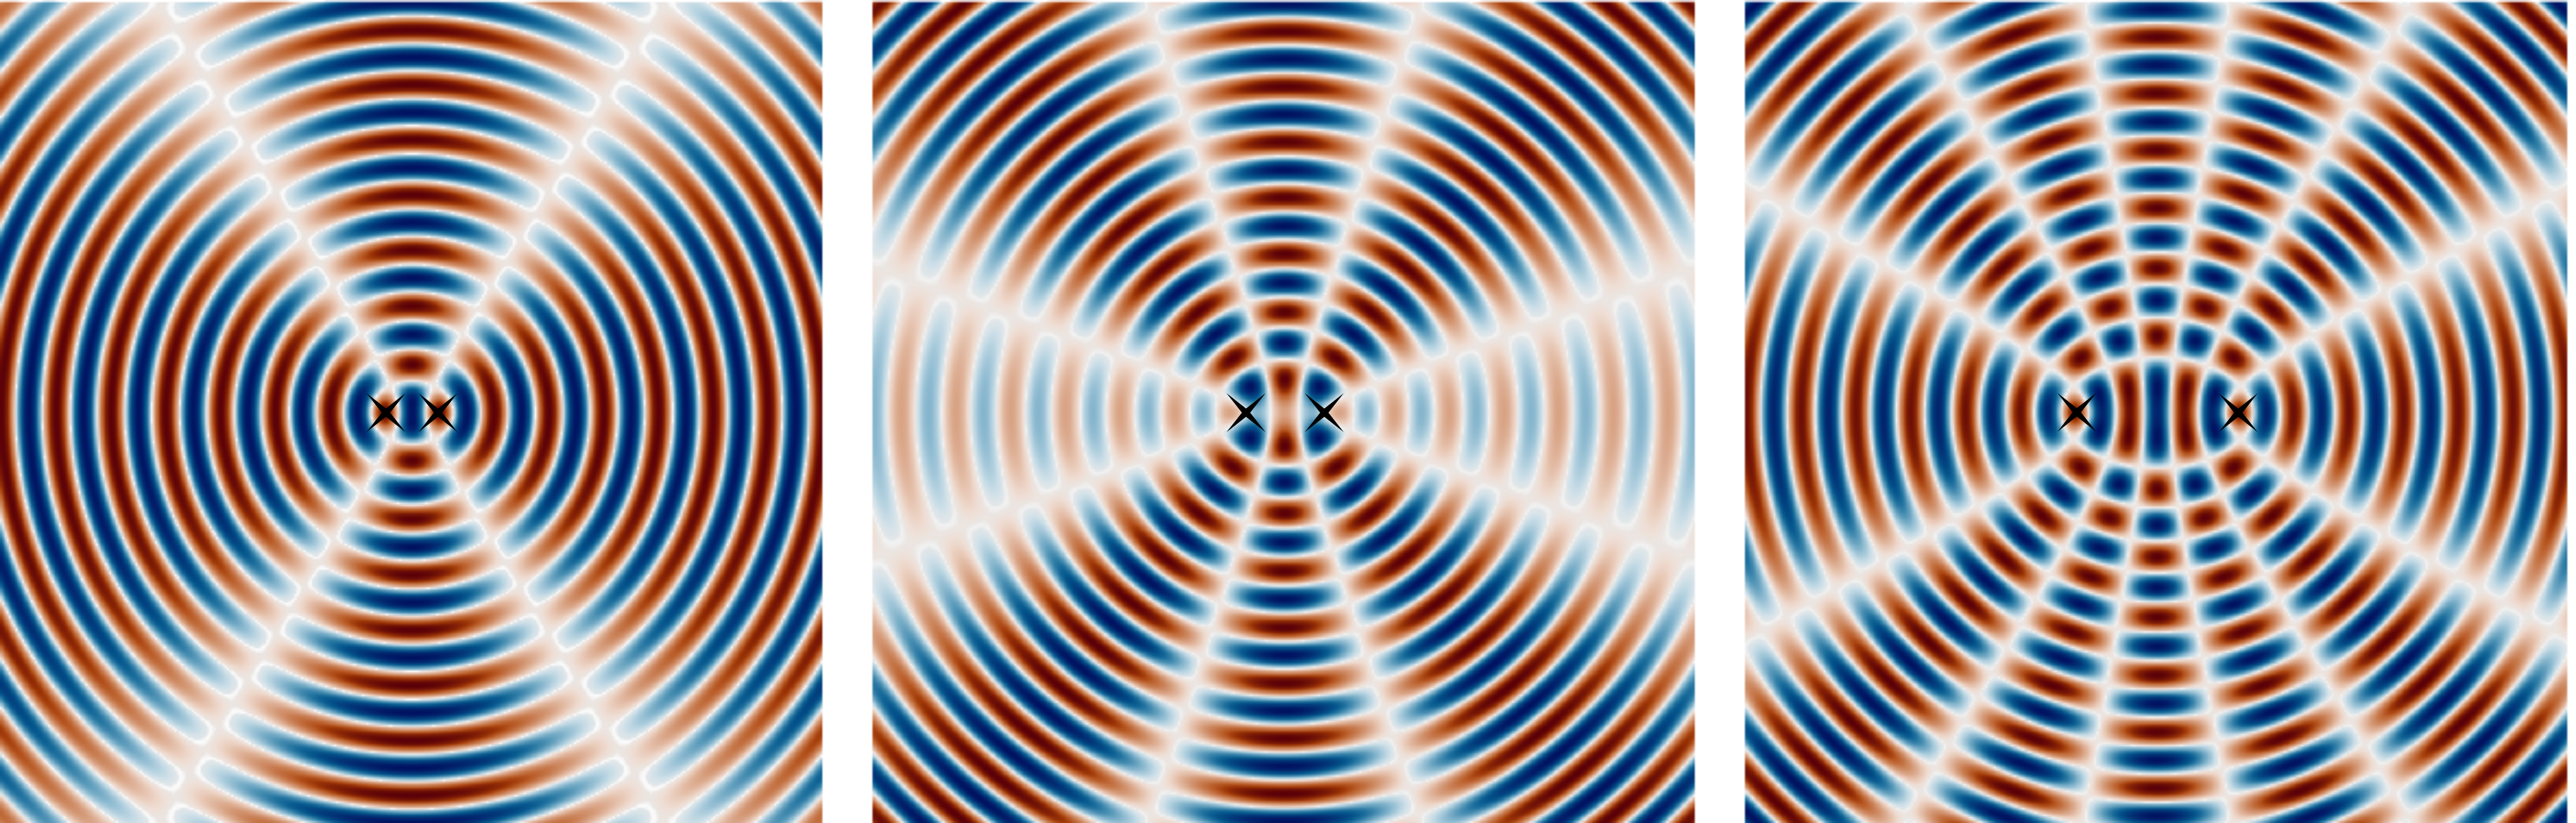
\includegraphics[width=140truemm]{slike/06_interferenca_krog.png}
\caption{Interferenca dveh krožnih valov za različne razmike med točkastima izvoroma. Kjer sta
valovanji iz faze (destruktivna interferenca), se pojavijo bele črte, ker sta valovanji v fazi
(konstruktivna interferenca), se pojavijo ojačitve. Z naraščajočim razmikom se ojačitve in oslabitve
gostijo.}
\label{fig:06_intkrog}
\vglue-5truemm
\end{figure}

\end{example}

\section{Interferenca z delitvijo valovne fronte}
V večini interferometričnih naprav in pri večini interferenčnih poskusov
ustvarimo interferenco z enim samim snopom svetlobe, 
ki ga razdelimo na dva dela. To lahko naredimo na dva načina: lahko razdelimo
valovno fronto valovanja (npr. Youngov poskus) ali pa razdelimo amplitudo
valovanja (npr. Michelsonov interferometer). 

Najpomembnejši primer interference z delitvijo valovne fronte je nedvomno
Youngov poskus (1801), na podlagi katerega je angleški fizik Thomas Young
spoznal, da je svetloba transverzalno valovanje. Pri tem poskusu vpadno valovanje iz 
monokromatskega izvora  
simetrično usmerimo na zaslon, v katerem sta dve enaki ozki
reži, in opazujemo sliko na oddaljenem zaslonu\footnote{Vpadno valovanje mora biti 
kar se da koherentno. Young je to dosegel tako, da je vpadno svetlobo najprej 
speljal skozi tanko režo in jo šele nato usmeril na zaslon z dvema režama. 
Več o koherenci bomo spoznali v poglavju~\ref{chap:Koherenca}.}. Poiščimo lego ojačitev in oslabitev
na oddaljenem zaslonu.
\begin{figure}[ht]
\centering
\def\svgwidth{120truemm} 
\input{slike/06_Young.pdf_tex}
\caption{Pri Youngovem poskusu svetloba prehaja ozko režo in vpada simetrično na dve ozki
reži. Na oddaljenem zaslonu opazujemo interferenco.}
\label{fig:06_Young}
\end{figure}

Naj bodo $z_0$ razdalja od objektnega zaslona z dvema režama 
do opazovalnega zaslona, $D$ razdalja med središčema rež, 
$r_1$ razdalja med sredino prve reže in izbrano točko na zaslonu
ter $r_2$ razdalja med sredino druge reže in točko na zaslonu. Potem za velike 
oddaljenosti $r_1, r_2 \gg D$ velja:
\beq
\Delta r = r_1-r_2 \approx D \sin\vartheta,
\label{eq:06_16}
\eeq
pri čemer je $\vartheta$ kot med osjo $z$ in zveznico med točko na sredini med režama in
izbrano točko na opazovalnem zaslonu. Uporabimo enačbo~(\ref{eq:06_09}) in za gostoto 
svetlobnega toka na zaslonu dobimo:
\beq
j = 4 j_0 \cos^2\left(\frac{\Delta \phi}{2}\right) = 4j_0 \cos^2\left(\frac{k\Delta r}{2}\right) = 
4j_0 \cos^2\left(\frac{kD\sin \vartheta}{2}\right)\!\!.
\label{eq:06_17}
\eeq

V točkah, kjer se prispevka obeh valovanj seštevata, nastopi tako imenovana
konstruktivna interferenca in na zaslonu opazimo ojačitve. Izhajajoč iz enačbe~(\ref{eq:06_17})
pogoj za ojačitev zapišemo kot:
\beq
\frac{kD\sin \vartheta}{2} = N\pi,
\label{eq:06_18}
\eeq
pri čemer je $N$ celo število. Od tod izračunamo pogoj za kote $\vartheta_\mathrm{max}$, pri katerih
se pojavijo vrhovi:
\boxeq{eq:InterferencaMax}{
D \sin\vartheta_\mathrm{max} = N \lambda.
}
Ker je leva stran enačbe enaka razliki poti od rež do točke na zaslonu, je zapis preprosto razumeti. 
Ojačitve se pojavijo, kjer je razlika poti od središč rež do točke na zaslonu enaka večkratniku 
valovne dolžine valovanja.

V vmesnih točkah, kjer se prispevka valovanj odštevata, je destruktivna
interferenca in na zaslonu opazimo oslabitve (temne proge). Pogoj za oslabitve je:
\boxeq{eq:InterferencaMin}{
D \sin\vartheta_\mathrm{min} = \left(N + \frac{1}{2}\right)\lambda.
}
Vzorec, ki se pojavi v daljnjem polju oziroma na oddaljenem zaslonu,
je za majhne kote periodičen s periodo ponavljanja $\Delta \xi_0$. Izračunajmo jo. Velja:
\beq
\Delta \left(\frac{kD\sin \vartheta}{2}\right) = \pi.
\label{eq:06_19}
\eeq
Za majhne kote $\vartheta$ velja 
\beq
k D \Delta \vartheta = k D \frac{\Delta \xi_0}{z_0} = 2 \pi,
\label{eq:06_20}
\eeq
od koder sledi:
\beq
\Delta \xi_0 = \frac{\lambda z_0}{D}.
\label{eq:06_21}
\eeq
Bliže kot so reže (manjši $D$), bolj razmaknjeni so uklonski vrhovi (večji $\Delta \xi_0$),
kar je seveda v skladu z uklonsko sliko. Za $D=1~\si{\micro\metre}$ je na oddaljenosti 
$z_0 = 1~\si{m}$ razmik med ojačitvami
$\Delta \xi_0 = 0,5~\si{m}$, medtem ko je pri $D = 1~\si{mm}$ 
vrednost $\Delta \xi_0 = 0,5~\si{mm}$. 

Pokažimo, da je dobljeni rezultat (enačba~\ref{eq:06_17}) enak tistemu, 
ki smo ga izpeljali pri obravnavi Fraunhoferjevega uklona v petem poglavju. 
Za sistem $N$ rež širine $d$ s periodo ponavljanja $D$ je veljalo 
(enačba~\ref{eq:uklonNrez}):
\beq
j(\vartheta) = j_0 \left(\frac{\sin\left(kd\sin\vartheta/2\right)}{kd\sin\vartheta/2}\right)^2
\left(\frac{\sin\left(NkD\sin\vartheta/2\right)}{\sin\left(kD\sin\vartheta/2\right)}\right)^2\!\!.
\label{eq:06_22}
\eeq
Uporabimo zapisano enačbo na primeru, ko je $N=2$, reži pa sta tako ozki, da lahko 
privzamemo $d\to 0$. Potem je strukturni faktor (prvi oklepaj) enak $1$ in 
intenziteta vrhov z oddaljenostjo od optične osi $z$ ne pojema. Ostane:
\beq
j = j_0~\frac{\sin^2(2kD\sin\vartheta/2)}{\sin^2(kD\sin\vartheta/2)} = 
j_0~\frac{4 \sin^2(kD\sin\vartheta/2)\cos^2(kD \sin\vartheta/2)}{\sin^2(kD \sin\vartheta/2)},
\eeq
pri čemer smo uporabili izraz za zapis dvojnega kota. Ulomek krajšamo in dobimo:
\beq
j = 4j_0 \cos^2\left(\frac{kD \sin\vartheta}{2}\right)\!\!,
\label{eq:06_23}
\eeq
kar je enako enačbi~(\ref{eq:06_17}).

\begin{remark}
Oglejmo si še nekaj alternativnih postavitev interferometrov z delitvijo žarka. Pri Youngovem
eksperimentu se namreč težko izognemo težavam, povezanim s končno širino reže $d$. Njegovi
sodobniki so poskušali podoben interferenčni vzorec ustvariti nad druge načine. Prvi primer
je Lloydovo zrcalo (1834), pri katerem interferirajo žarki, ki pridejo neposredno od izvora svetlobe, 
in žarki, ki se odbijejo od zrcala. Drugi primer sta Fresnelovi zrcali, pri katerih interferirata
sva snopa svetlobe, ki se odbijata vsak od svojega zrcala. Tretja postavitev, ki jo omenimo,
je s Fresnelovo biprizmo. Svetloba, ki izhaja iz enega svetila, se na Fresnelovi biprizmi
lomi, lomljena žarka pa med seboj interferirata.

\begin{figure}[ht]
\centering
\def\svgwidth{140truemm} 
\input{slike/06_Lloyd.pdf_tex}
\caption{Različne postavitve za opazovanje interference: Lloydovo zrcalo (a), Fresnelovi
zrcali (b) in Fresnelova biprizma (c). Črtkane črte označujejo navidezne izvore svetlobe.}
\label{fig:06_Lloyd}
\end{figure}
\vskip1truecm
\end{remark}

\section{Interferenca z delitvijo amplitude}
\label{chap:Michelson}
Amplitudno delitev valovanja dosežemo s polprepustnimi zrcali. Kot že ime pove, taka
zrcala del vpadne svetlobe odbijejo in del prepustijo. 
Najznačilnejši primer interferometra z delitvijo amplitude je Michelsonov interferometer.
Z njim je Michelson pokazal, da je hitrost svetlobe v smeri gibanja Zemlje enaka hitrosti
svetlobe v smeri pravokotno na smer gibanja in tako ovrgel teorijo o obstoju etra. 

V Michelsonovem interferometru vpadno svetlobo s polprepustnim zrcalom razdelimo 
na dva snopa. Delna snopa usmerimo na  vsak od svojega zrcala in interferirata na detektorju. 
S premikanjem enega od zrcal spreminjamo
zakasnitev med žarkoma in na detektorju se izmenično pojavljajo ojačitve in oslabitve.
Gostota svetlobnega toka na detektorju je (enačba~):
\beq
j = 4j_0 \cos^2(\Delta \phi/2),
\label{eq:06_24}
\eeq
pri čemer je $\Delta \phi = k_0(l_1-l_2)$....


\section{Interferenca na tanki plasti}
Do zdaj smo obravnavali interferenco, pri kateri je bilo skupno valovanje sestavljeno iz le 
dveh prispevkov. Zdaj si oglejmo primer interference, ki nastane kot vsota zelo velikega 
števila delnih valovanj. 

Naj ravno valovanje vpada na tanko plast snovi z lomnim količnikom $n_2$, lomni količnik 
okolice pa naj bo enak $n_1$, pri čemer se omejimo na primer TE polariziranega valovanja.
Ob vpadu na plast se del svetlobe odbije, del pa lomi v snov po lomnem zakonu (enačba~) 
z amplitudo, ki jo določa Fresnelova enačba (). Prepuščeni val potuje po plasti do meje
na drugi strani, kjer je ga ponovno nekaj odbije, del pa je prepuščen v smeri, ki 
je enaka vpadni smeri. Odbiti del valovanja potuje 
do vpadne meje, kjer se deloma odbije, del pa ga izhaja na vpadni strani ... 

Jakost prepuščenega električnega polja je tako sestavljena iz velikega števila prispevkov, ki 
izhajajo v isti smeri, njihove amplitude pa so vedno manjše. Ker izhodni žarki 
izhajajo na različnih točkah, jih navadno z zbiralno lečo preslikamo v eno točko. Pri pravokotnem
vpadu na tanko plast teh težav ni. 

Zanima nas gostota prepuščenega svetlobnega toka $j$ v odvisnosti od 
lomnih količnikov $n_1$ in $n_2$, vpadnega kota $\alpha$ in debeline plasti $d$. 

Najprej z lomnim zakonom izračunamo kot $\beta$, pod katerim se širi svetloba v plasti:
\beq
\sin\beta = \frac{n_1}{n_2}\sin\alpha.
\label{eq:06_25}
\eeq
Amplitudna odbojnost $r$ in prepustnot $t$ na prvi meji sta enaka (enačba~):
\beq
r_{12} = \frac{n_1\cos \alpha - n_2\cos \beta}{n_1\cos \alpha + n_2\cos \beta}\qquad 
\mathrm{in}\qquad t_{12} = 1+r_{12},
\label{eq:06_26}
\eeq
na drugi meji pa:
\beq
r_{21} = \frac{n_2\cos \beta - n_1\cos \alpha}{n_2\cos \beta + n_1\cos \alpha}\qquad 
\mathrm{in}\qquad t_{21} = 1+r_{21}.
\label{eq:06_27}
\eeq
Vidimo, da velja $r_{12} = r_{21}$. Ko poznamo vse koeficiente, lahko zapišemo
posamezne prispevke jakosti električnega polja na prepuščeni strani:
\begin{align}
E_1 &= E_0\,t_{12}\,t_{21},\\
E_2 &= E_0\,t_{12}\,r_{21}\,r_{21}\,e^{i\phi}\,t_{21},\\
E_3 &= E_0\,t_{12}\,r_{21}\,r_{21}\,e^{i\phi}\,r_{21}\,r_{21}\,e^{i\phi}\,t_{21},\\
&...\\
E_{N+1} &= E_0\,t_{12}\,\left(r_{21}\,r_{21}\right)^N\,e^{iN\phi}\,t_{21}\\
&...
\label{eq:06_29}
\end{align}

\begin{figure}[ht]
\centering
\def\svgwidth{140truemm} 
%\input{slike/06_.pdf_tex}
\caption{SLIKA}
\label{fig:06_Nrez}
\end{figure}

Pri tem smo upoštevali tudi fazni zamik zaradi dodatne prepotovane poti v plasti:
\beq
\phi = k_0 2d \cos \beta n_2.
\label{eq:06_31}
\eeq
Dodaj izpeljavo, skico. 
Celotno polje zapišemo kot vsoto vseh teh prispevkov:
\begin{align}
E_t &= E_1+E_2+E_3+... + E_N + ... \\
& E_0\, t_{12}\,t_{21}\,\left(1 + r_{21}^2 e^{i\phi} + r_{21}^4 e^{2i\phi} + r_{21}^6 e^{3i\phi} + ... \right).
\label{eq:06_30}
\end{align}
Geometrijsko vrsto lahko seštejemo in za prepuščeno polje dobimo:
\beq
E_t = \frac{E_0 t_{21}t_{12}}{1-r_{21}^2e^{i\phi}} = E_0 t.
\label{eq:06_32}
\eeq
Zanima nas gostota prepuščenega energijskega toka glede na vpadno. Ker sta lomni količnik snovi
in smer širjenja svetlobe na izhodni strani enaka kot na vpadni, je prepustnost $T$ kar enaka $|t|^2$.
Uporabimo enačbo~(\ref{eq:06_32}) in upoštevamo zveze med amplitudnimi prepustnostmi in odbojnostmi:
$t_{21} = 1+r_{21} = 1-r_{12}$ in $t_{12} = 1+r_{12}$. Vpeljemo odbojnost $R = r_{12}^2 = R$.
Prepustnost je tako:
\beq
T
\label{eq:06_33}
\eeq



\section{Fabry-Perotov interferometer}

\section{Večplastni nanosi}
